\chapter{Experiments}

In the experimental phase, we selected datasets that have previously been utilized in well-recognized competitions. This allows us to benchmark the 
performance of our model against established baselines and leading-edge results within the field, helping us make meaningful comparisons with our model. 
Each dataset employed in our experiments represents a common scenario in the field of object detection, encompassing diverse environments and perspective 
urban life captured through ground-level cameras, aerial views provided by drones, and wide-ranging perspectives from satellites. 

\section{Datasets}
For the benchmarking of our model we decided to use three very well known datasets, and we are going to analyze in this section.


\subsection{Microsoft Common Object in COntext (MS COCO)}
The Microsoft Common Objects in Context (MS COCO) dataset 2017 is a comprehensive image dataset designed for object detection, segmentation, and captioning tasks. 
It is known for its complexity of its images, which are primarily sourced from everyday scenes. The dataset includes 80 object categories, providing a wide 
range of common objects for robust training and evaluation of machine learning models. These categories encompass various items from person, bicycle, 
car, to stop sign and smaller objects like toothbrush.

In terms of its composition, the MS COCO 2017 dataset contains over 118,000 training images, 5,000 validation images, and a test set of around 41,000 images, 
bringing its total to approximately 164,000 images. This dataset is also accompanied by over 1.5 million object instances, each annotated. 
The annotations are formatted to support both object detection and instance segmentation tasks. Specifically, for object detection, each annotation includes 
not only the class label and a bounding box defined by the $x$ and $y$ coordinates of the top-left corner, width, and height, but also a detailed segmentation 
mask for each object instance, making it suitable for more granular segmentation tasks as well.

The dataset is divided into training, validation, and test splits to facilitate the training and fine-tuning of models in a structured manner. 
This split ensures that models can be trained on a large set of images and parameters can be fine-tuned on the validation set before final evaluations 
are performed on the test set. The use of MS COCO for competition and research has helped advance the field of computer vision by providing a challenging 
set of images and annotations that test the limits of both existing and novel visual recognition models.

Class Distribution in COCO 2017:

\begin{figure}[h!]
    \centering
    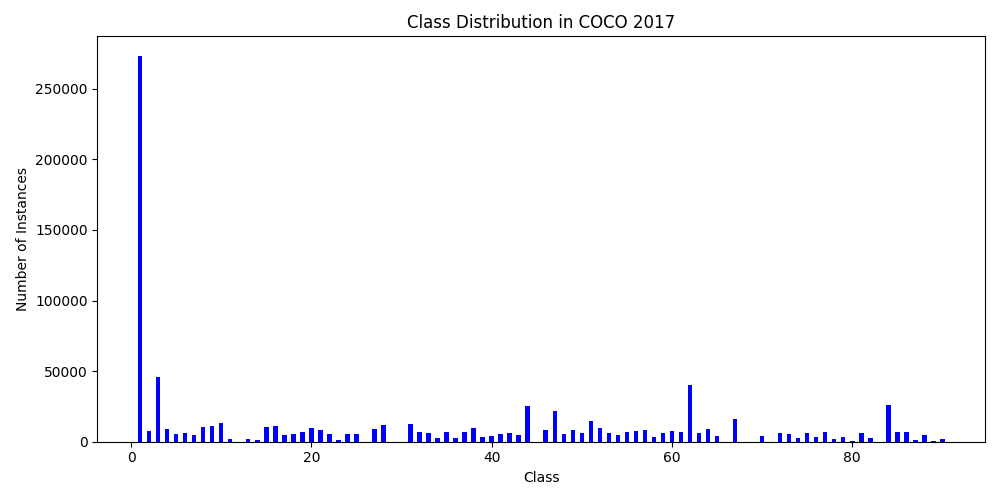
\includegraphics[scale=0.55]{Figures/coco2017_class_distribution.png}
    \caption{Class Distribution in COCO 2017}
    \label{fig:coco-class}
\end{figure}

\subsection{Unmanned Aerial Vehicle Small Object Detection}

The UAV-SOD (Unmanned Aerial Vehicle Small Object Detection) dataset is specifically designed for advancing research in the area of object detection using 
aerial imagery captured by drones. This dataset focuses on the detection of small objects, which presents unique challenges due to the small scale and often 
complex backgrounds seen in aerial images. Here are the key details about the UAV-SOD dataset. The UAV-SOD dataset includes detailed annotations for each image, 
essential for supervised machine learning models such as object detectors. Annotations are provided in XML format compatible with the PASCAL VOC annotation 
format, which is widely used in object detection tasks. These annotations include bounding boxes that specify the coordinates of each object in the image. 
The objects in this dataset are annotated with their class labels, enabling not only object detection tasks but also potential use for object classification 
and segmentation challenges.

Class Distribution in UAV Small Object Detection:

\begin{figure}[h!]
    \centering
    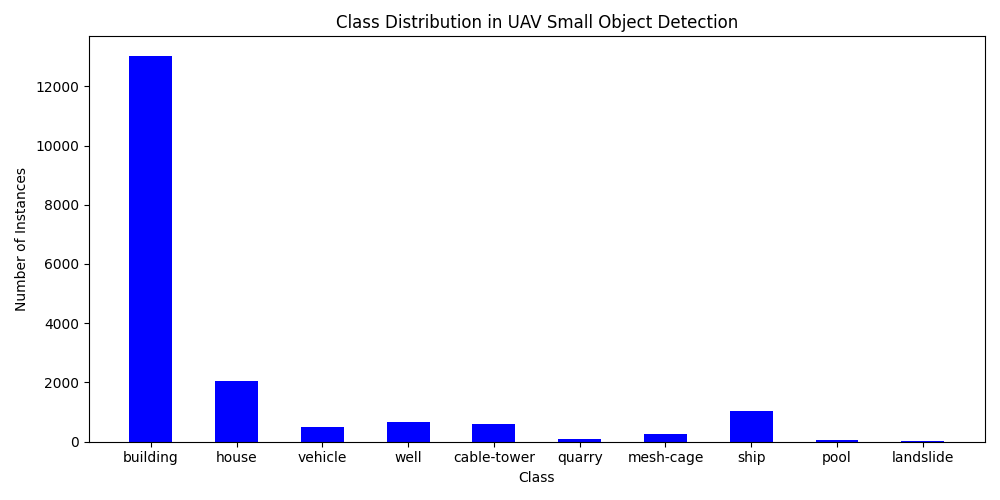
\includegraphics[scale=0.55]{Figures/uav_sod_data_class_distribution.png}
    \caption{Class Distribution in UAV Small Object Detection}
    \label{fig:uav-class}
\end{figure}


\subsection{VisDrone}

VisDrone is a dataset designed for drone-based object detection, featuring $10,209$ images captured across various environments using different 
types of drones. Each image in the dataset has a high resolution of $2000 \times 1500$ pixels. The dataset is organized into splits for comprehensive 
training and evaluation, consisting of $6,471$ images for training, $548$ images for validation, and $3,190$ images for testing. VisDrone includes a 
diverse set of ten object classes, such as pedestrians, cars, vans, buses, trucks, motorcycles, bicycles, awning-tricycles, and tricycles. This wide 
range of categories, combined with the diverse aerial perspectives provided by drone capture, makes VisDrone an ideal resource for developing and 
benchmarking deep learning models focused on enhancing object detection capabilities in drone surveillance systems.

Class Distribution in VIS Drone:

\begin{figure}[h!]
    \centering
    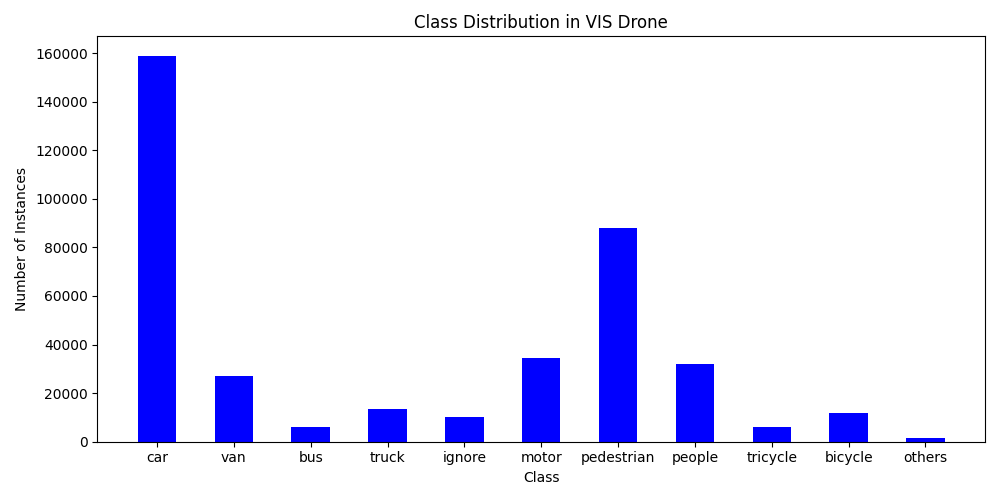
\includegraphics[scale=0.55]{Figures/vis_drone_data_class_distribution.png}
    \caption{Class Distribution in VIS Drone }
    \label{fig:vis-class}
\end{figure}


\section{Data Pre-Processing}





\section{Evaluation Metrics}



\section{Training}



